% TEX STUDIO MAGIC-COMMAND
% !TeX document-id = {21ffa6e2-6c8f-4532-897c-386dc477f19a}
% !TeX root = abstract.tex
% !TeX encoding = utf8
% !TeX TXS-program:compile = lualatex -file-line-error -synctex=1 -interaction=nonstopmode -halt-on-error %.tex
% !TeX TXS-program:quick = txs:///compile | txs:///view-pdf-internal --embedded
%%% TeXのファイル名を変えたら ↑ も変えましょう



%%%-------------------------------------------------------------------------
%%% PD3予稿集テンプレート (main.tex)
%%% 作成: 金沢工大・情報工学科・鷹合研究室(2022,01/12)
%%%-------------------------------------------------------------------------

%%%%%%%%%%%%%%%%%%%%%%%%%%%%%%%%%%%%%%%%%%%%%%%%%%%%%%%%%%%%%%%%%%%%%%%%%%%
%                               テーマ,著者情報をここに書き込んでください
%ここから ------------------------------------------------------------------

%%% テーマ番号
\def\THEMEID{1EP001}

%%% タイトル
\def\TITLEJP{機械学習用いた電車の車両タイプの判別システムの開発}
\def\TITLEEN{Development of a train car type identification system using machine learning}
\def\CENTERADJ{3.3} % ここを書き換えて,表紙の「プロジェクトテーマ」という文字列がセル中心になるよう調整してください

%%% 教員名
\def\PROFNAME{鷹合 大輔 准教授}

%%% アブストラクト(英文で書く)
% 最低:100ワード,最大:300ワード前後
% 英文部分については,句読点は半角にすること.つまり", "か". "を使う
\def\ABSTRACT{
Describe about 5 lines of abstract in English here. Describe about 5 lines of abstract in English here. Describe about 5 lines of abstract in English here. Describe about 5 lines of abstract in English here. Describe about 5 lines of abstract in English here. Describe about 5 lines of abstract in English here. 
\textbf{(何が問題で,それをどんな手法で取り組んで,どういう結果であったかなどを英語で要約して下さい)}
 Describe about 5 lines of abstract in English here. Describe about 5 lines of abstract in English here. Describe about 5 lines of abstract in English here.
}

%%% キーワード(5個まで)
\def\KEYWORDS{YOLO,Machine Learning,Qwerty3,Qwerty4,Qwerty5}

%%% 著者リスト
\def\AUTHORS{
\begin{minipage}{13.5cm}
~\hfill 4EP1-68~野崎 悠渡(NOZAKI Yuto)      ~~~~~ 4EP5-11~田村 優祐(TAMURA Yusuke) \hfill~
\end{minipage}
}

\newcommand{\red}[1]{\textcolor{red}{#1}}


% テーマ,著者情報ここまで -----------------------------------------------------


%%%%%%%%%%%%%%%%%%%%%%%%%%%%%%%%%%%%%%%%%%%%%%%%%%%%%%%%%%%%%%%%%%%%%%%%%%%%
%                                本文


\documentclass{tkglabs}

\usepackage{caption}

\begin{document}
\maketitle
\begin{multicols*}{2} % *アスタ付きだとページのバランシングを無効にできる
%本文ここから ------------------------------------------------------------------



\section{はじめに}
%背景や目的をここに書いてください.
電車の車両タイプはJRの在来線だけでも100種類近く存在している.
電車を見て電車だと認識することは可能だが,その電車の車両タイプまでを判別できる人は少ない.
電車の知識がある人は一目見るだけでその電車の車両タイプを判別できるが,電車の知識があまりない人は似ている電車の車両タイプを判別することが難しい.本プロジェクトでは簡単に画像や動画に写っている車両タイプが何なのかを判別できるシステムを開発する.

%\section{関連研究?現存するサービスについて?これいる??}
%先行事例と本システムの独自性
%googleがgoogleレンズというサービスを提供している.これは,画像に写っている物体と同じものが写っているウェブサイトをまとめて表示するサービスである.このサービスの問題点は3つある.
%\begin{itemize}
%	\item 一枚の画像に複数の物体が写り込んでいると判別結果が正確ではなくなる.
%	\item 提示されたウェブサイトから詳細を確認しなければならない.
%	\item 動画から物体を判別することができないこと
%\end{itemize}

\section{システム概要}
%開発するシステムの概要を図 \ref{abc}に示す.
本システムは,ユーザに画像ないしは動画をブラウザ上で入力してもらい,それをサーバ上で画像認識を用いて処理し,結果をブラウザで表示するWebアプリケーションである.システム概要を図\ref{abc}に示す.
\begin{figure} % 小さな図
	\label{abc}
	\centering
	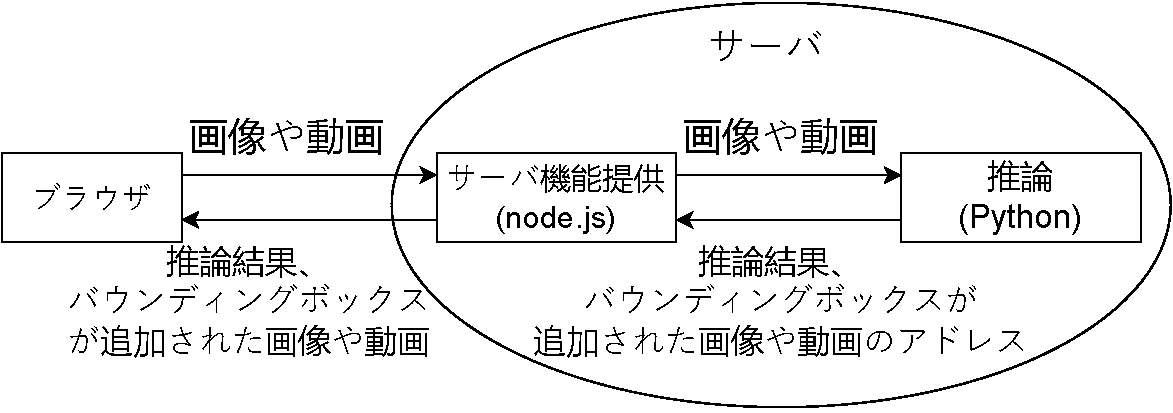
\includegraphics[width=\linewidth]{obj/sys_gaiyou1.pdf}
	\figcap{システム概要}{System Overview}{abc}
\end{figure}


\section{判別モデルの開発の流れ}
電車が写っている画像を集めて,データセットを作成し,学習をするという流れで判別モデルを開発する.

\subsection{データ収集}
	YouTubeで特定の電車のみが映っている1〜3種類の動画を保存して,指定した枚数分のランダムなフレームを保存する.保存した画像を識別して,	電車が映っている画像だけを保存する.
	%動画ごとに電車が写っている時間が異なるため,集めた画像は車両タイプごとに異なる.
	%各車両タイプが名前になっているディレクトリに保存する.
各車両タイプの画像の保存枚数を図\ref{fig:chart}に示す.

% TODO: \usepackage{graphicx} required
\begin{figure}
	\centering
	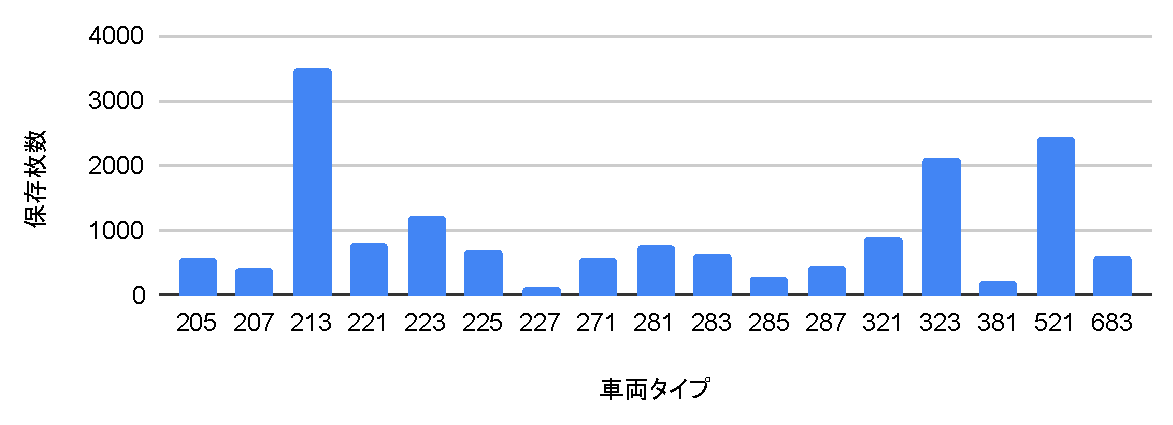
\includegraphics[width=\linewidth]{obj/chart1.pdf}
	\figcap{各車両タイプの保存枚数}{aaa}{fig:chart}
\end{figure}
\subsection{データセットの作成}
本プロジェクトで作成するモデルは識別モデル,分類モデルの二種類である.%データセットのディレクトリ構造が識別用と分類用で異なるので,それぞれのデータセットを作成した.識別モデルには画像のアノテーション情報も必要なので,アノテーションを行い,識別モデル用のデータセットを作成した.
分類モデルのデータセット内の画像をアノテーションして,識別モデル用のデータセットを作成した.
様々なウェブサイトから手作業で17種類の各車両の画像を10枚ずつ集めて,テストデータセットを作成した.

\subsubsection{分類と識別について}
分類はデータやオブジェクトを異なるクラスやカテゴリに分けるプロセスを指す.画像の分類とは,画像が特定のカテゴリやクラスに属するかどうかを判別する作業である.例えば,画像に写っているのが猫か犬かのクラスに分けることである.

識別とは画像のどこに何が写っているのかを判別するプロセスを指す.1枚の画像に複数の物体が存在する場合も識別はできる.動画上の車両タイプも判別することができる.


\subsection{モデルの学習}
%本プロジェクトでは\\
作成したデータセットとYOLOv8を用いてモデルの学習を行い2種類のモデルを作成した.
分類モデルでは画像での判別しかできない.動画から車両タイプを判別するために識別モデルを作成した.

%\subsubsection{学習の実行}
%学習を進めると徐々に性能が上がっていき性能が向上しなくなると学習が途中で中断される.
%学習は中断されるまで続けたため,学習回数はモデルによって差がある.
%識別モデルと分類モデルをどのように使えば結果が出力されるのかを説明する.pythonのコードを貼り付ける?
%田村のパートに記載してもいいかもしれない


\section{システムの機能}
%本システムの機能として電車の分類と識別を提供する.識別は動画と画像の両方に対応している.
%画像や動画を入力すると,判別結果が出力される.
%本システムは,以下の3つの機能を提供する.
本システムは,電車の分類と電車の画像と動画の識別の3つ機能を提供する
%\begin{itemize}
%	\item 電車の画像の分類
%	\item 電車の画像の識別
%	\item 電車の動画の識別
%\end{itemize}

\subsection{電車の画像の分類} 
出力後の画面を図\ref{img_cls}に示す.
この機能では,ユーザがブラウザからアップロードした画像に含まれる電車の種類を分類する. 分類の結果,最も可能性が高いものをHTMLページに出力する.
\subsection{電車の画像の識別}
出力後の画面を図\ref{img_det}に示す.
この機能では,ユーザがブラウザからアップロードした画像に含まれる電車の位置と種類を識別する.  識別の結果,バウンディングボックスが追加された画像をHTMLページに表示する.
\subsection{電車の動画の識別} 
出力後の画面を図\ref{mov_det}に示す.
この機能では,ユーザがブラウザからアップロードした動画に含まれる電車の位置と種類を識別する. 識別の結果,バウンディングボックスが追加された動画をHTMLページに表示する.

%\begin{figure}
%	\centering
%	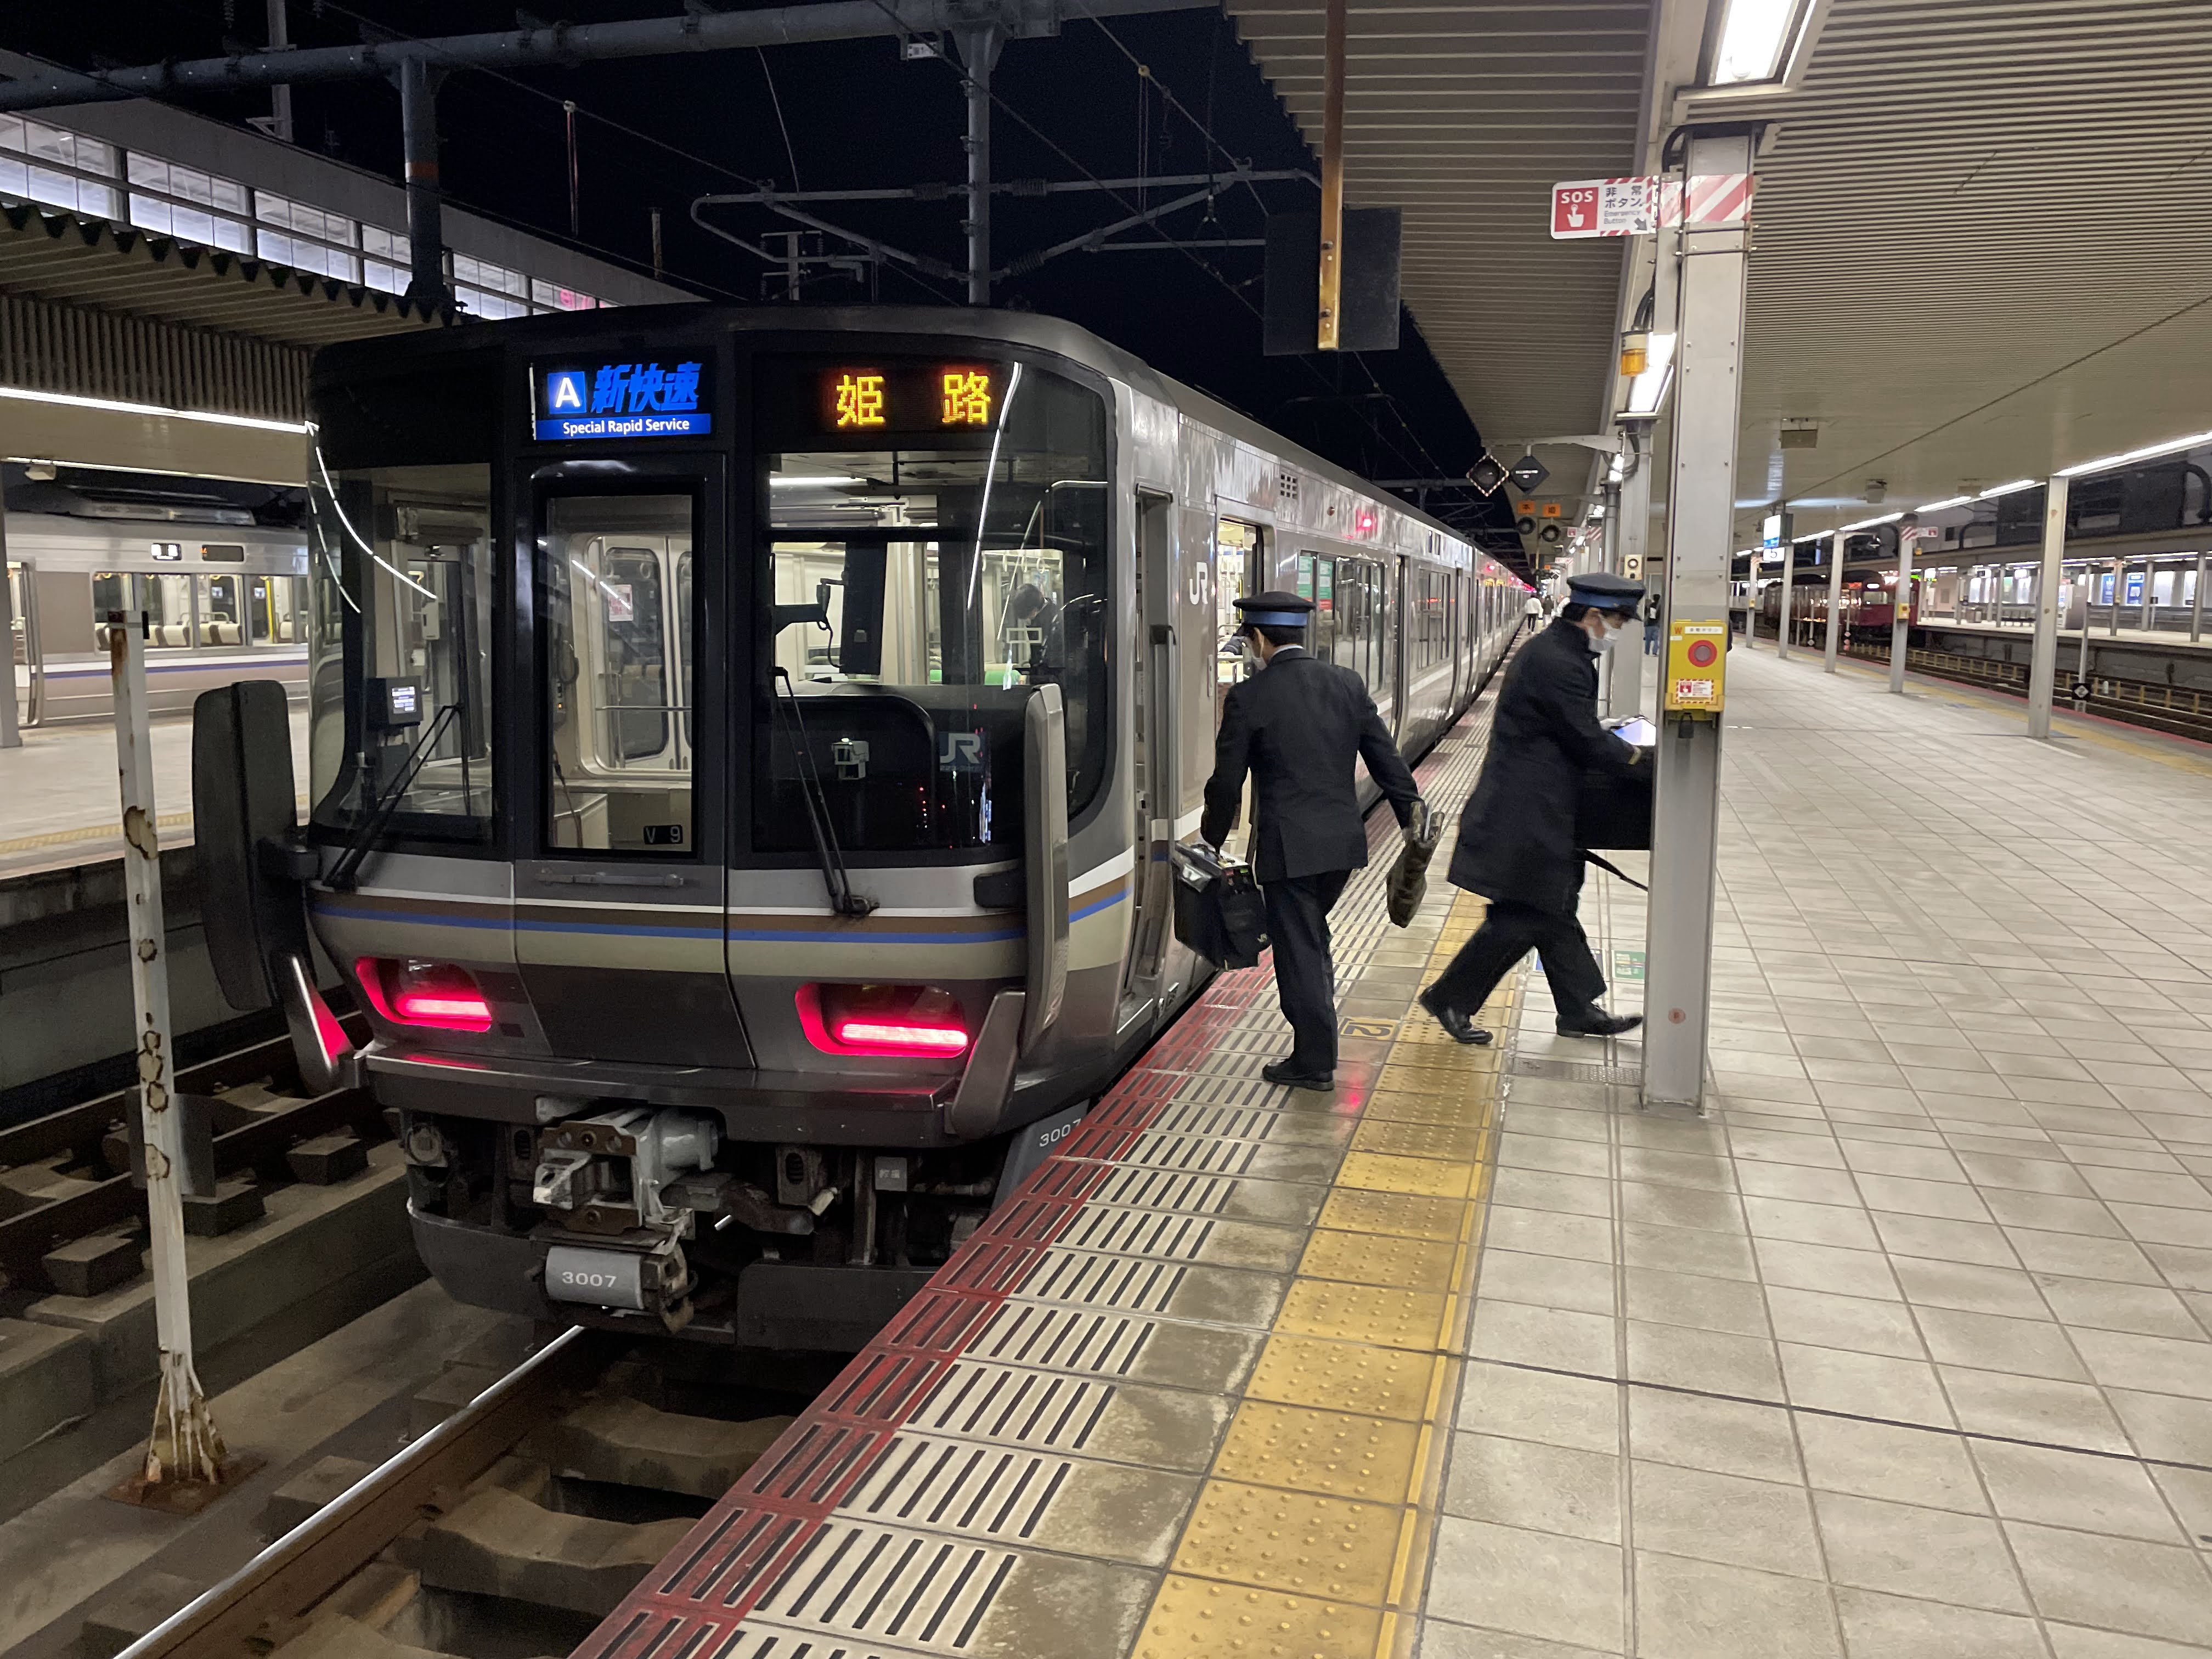
\includegraphics[width=0.5\linewidth]{obj/image1.png}
%	\figcap{画像の分類}{classify image}{cls-img}
%\end{figure}

\begin{figure}
	\begin{tabular}{ccc}
		\begin{minipage}[b]{0.3\textwidth}
			\centering
			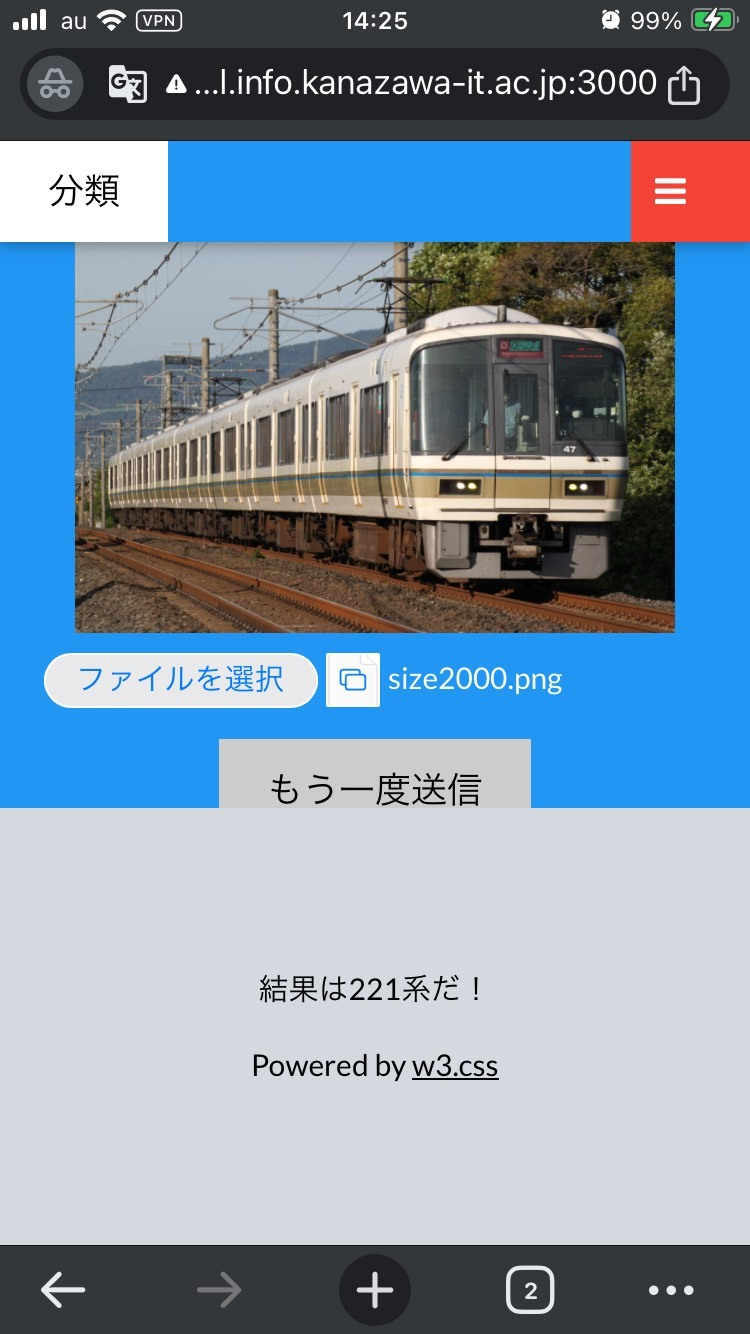
\includegraphics[width=\linewidth]{obj/img_classify.jpg}
			\figcap{画像の分類}{classify image}{img_cls}
		\end{minipage}
		\begin{minipage}[b]{0.3\textwidth}
			\centering
			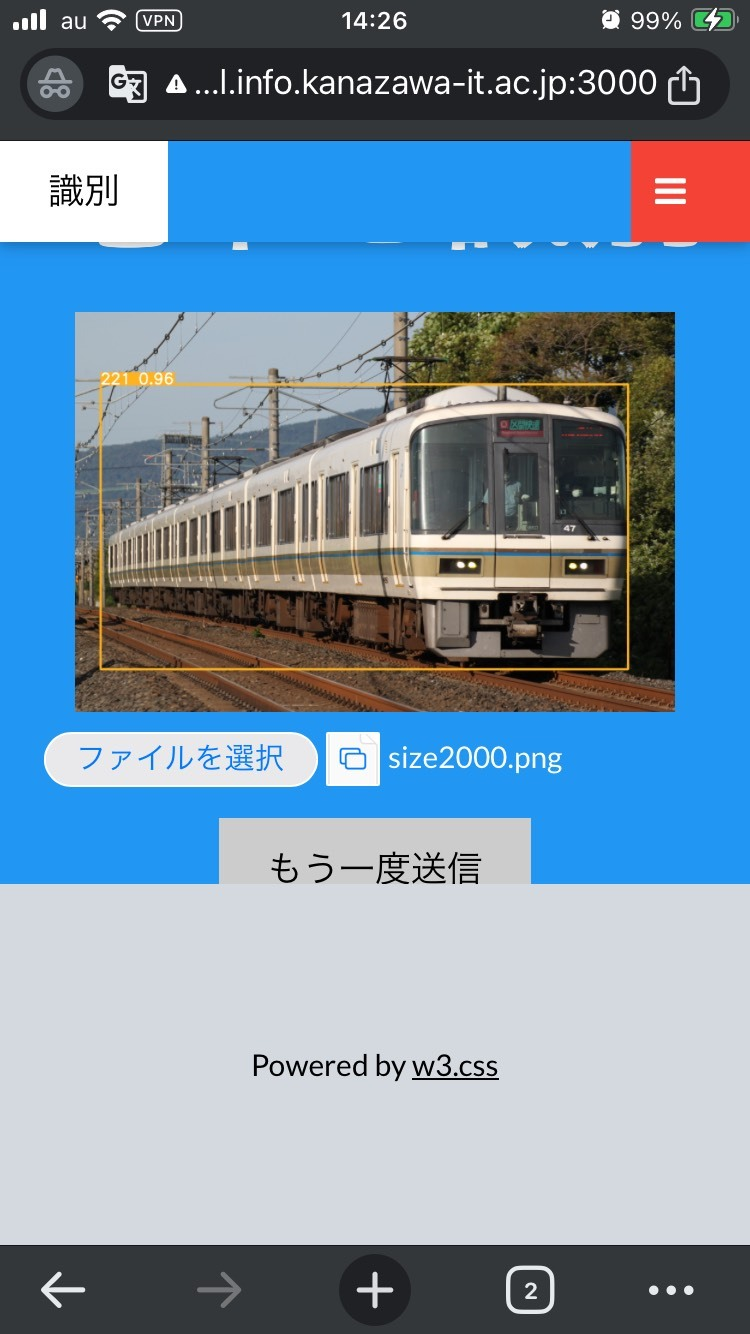
\includegraphics[width=\linewidth]{obj/img_identify.jpg}
			\figcap{画像の識別}{detection image}{img_det}
		\end{minipage}
		\begin{minipage}[b]{0.3\textwidth}
			\centering
			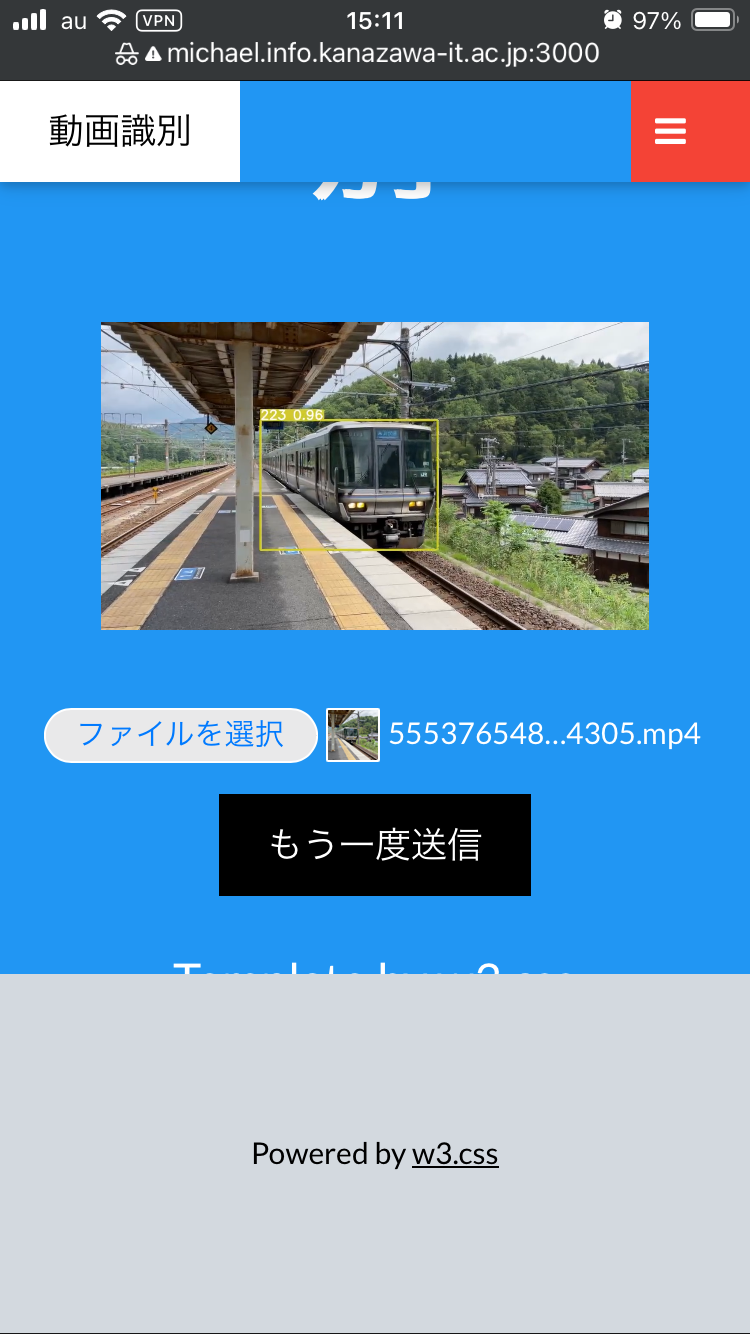
\includegraphics[width=\linewidth]{obj/mov_det.jpg}
			\figcap{動画の識別}{detection movie}{mov_det}
		\end{minipage}
	\end{tabular}

\end{figure}
%https://link-blog.hatenablog.com/entry/2022/10/15/192639を参照
\section{動作確認と現状}
学内ネットワークからWebアプリケーションに接続すると画像の分類,画像の識別,動画の識別の動作を確認できた.
スマホで4G回線に接続し,学内のVPNを用いた際にも動作したもののアップロードにかなりの時間を要した.その際にnode.jsのプログラムメモリ消費量が増大した.このことから,メモリリークが発生していると思われる.現状,弱い回線での接続をする際には注意が必要である.


%ここまで田村

ーーーーーーここまで田村ーーーーーーーー

\section{作成したモデルの評価}
%\subsection{モデルの性能評価指標}
%本プロジェクトで作成する分類モデルは混合行列から性能の評価を行う.混合行列とは実際のデータと予測データを比較するためのもので,正しくラベル設定ができているのか,及び予測の精確度を把握することができる.

\subsection{分類モデルの性能評価}
作成した分類モデルを用いてテストデータセットの分類を行った結果を図\ref{fig:classifyresults}に示す.
\begin{figure}
	\centering
	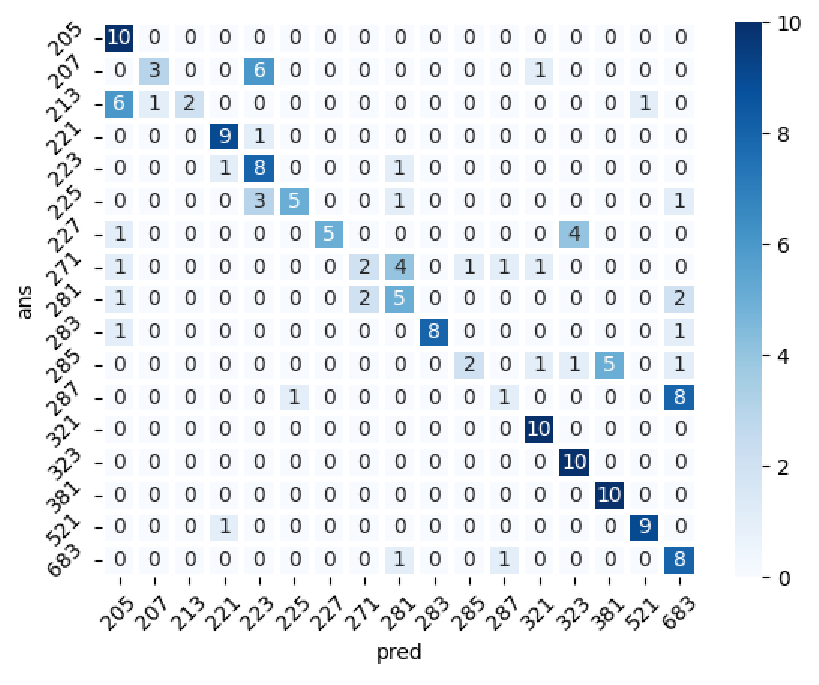
\includegraphics[width=\linewidth]{obj/classify_results.pdf}
	\figcap{性能評価}{seinouhyouka}{def}
	\label{fig:classifyresults}
\end{figure}

\subsection{識別モデルの性能評価}
%17種類の車両タイプの画像をそれぞれ10枚ずつ集めテストデータを作成し識別を行った.識別の結果を表\ref{detection}に示す.
%captionを追加するとエラーが発生してしまう
作成した識別モデルを用いてテストデータセットの識別を行った結果を図\ref{fig:chartdet}に示す.
識別失敗とは間違った車両タイプだと判断し,識別不能とはどの車両タイプにも当てはまらないと判断したことを指す.
% TODO: \usepackage{graphicx} required
\begin{figure}
	\centering
	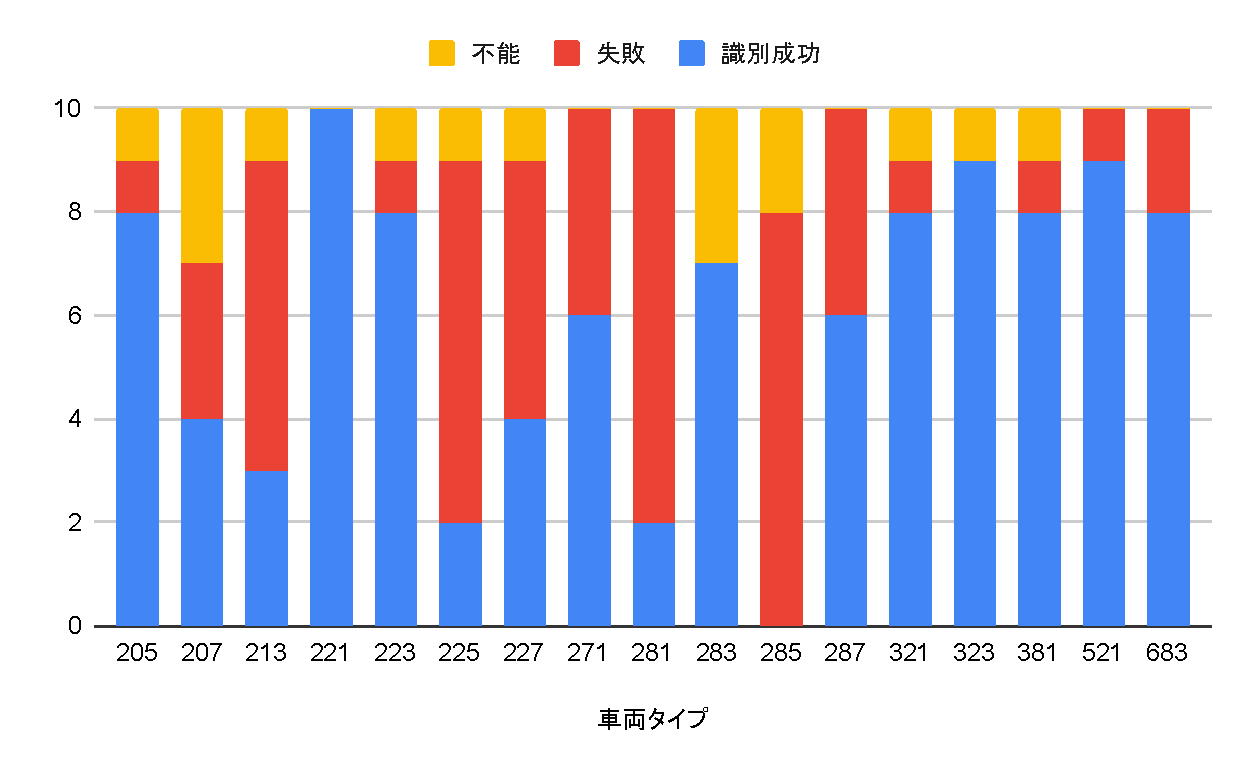
\includegraphics[width=\linewidth]{obj/chartDET.pdf}
	\figcap{テストデータ識別結果}{ababefn}{}
	\label{fig:chartdet}
\end{figure}





\section{作成したモデルの考察}
正解率は電車によって異なることがわかる.特に外見が似ている電車だと,誤判別していることが多かった.
%データセットの画質を落とすと誤判別が増えた.特に誤分類が多かった三種類の電車の画質を上げても結果はあまり変わらなかった.
%限られたストレージでは,データセットの画質を変化させて判別結果を向上させることは難しいと考えられる.SSDの容量に制限がない場合,大量の高画質のデータでデータセットを作成することで判別結果が改善される可能性があると考えられる.
%各車両タイプの画像の枚数に差があったことが判別結果に影響を与えていると考えられる.
データセットの画像の枚数が少ない車両タイプの判別結果が必ず悪くはならなかった.
画像の枚数が判別結果に影響を与えるのではなく,車体の特徴が鮮明に写っている画像の枚数が判別結果に影響を与えると考えられる.
判別精度の向上のために,データセットとして質の悪い画像を大量に集めるのではなく,車体の特徴が鮮明に写っている画像を車両タイプごとに集める必要があったと考えられる.



\section{まとめ}
本プロジェクトでは,機械学習を用いた電車の車両番号を判別するため,2種類のモデルを作成した.また,電車が写っている画像や動画をサーバ上で,分類,識別を行い判別結果を出力するウェブアプリを作成した.

モデルを学習させるためのデータセットは,動画から電車が写っている場面だけを保存して作成した.作成したモデルで車両タイプの判別をすると,外見が似ている電車の判別結果が悪く,外見に特徴のある電車の判別結果は良かった.その原因は,車体の特徴がうまく写っていない画像もデータセットに含まれていることだと考えられる.

電車の画像の分類,識別,動画の識別をする機能を持ったWebアプリケーションを作成することができた.電波の弱い場所以外では正常に動作することが確認できた.
%% 参考文献(必要に応じて追加)
\begin{thebibliography}{99}
%\bibitem{jp2k1} 織田 信長, 明智 光秀, "JPEG2000画像符号化システムにおける係数ビットモデリングと適応算術符号化,"Journal of signal processing(基礎シリーズ), vol.7, no.4, pp.257-266, July 2003.
%\bibitem{sdkguide}Parrot, "AR.Drone Developer Guide SDK 2.0"
%\bibitem{bk1} "金沢の暮らし", \url{http://www.kanazawa-it.ac.jp}
%\bibitem{bk2} 山田 太郎, "金沢の一人暮らし", トンチンカン出版, 2016.
%\bibitem{bk0}"Ultralytics YOLOv8 ドキュメント",\url{https://docs.ultralytics.com/ja}
%\bibitem{bk1}"アノテーションとは - 定義と重要性,必要な準備や注意点を解説",\url{https://www.dir.co.jp/world/entry/solution/annotation}
\end{thebibliography}

%\noindent\textbf{本プロジェクトに関する業績} % 学部
% \noindent\textbf{本研究に関する業績} % 院生の場合
%\begin{enumerate}[label=\arabic*),leftmargin=2.25\zw]
%\item 鈴木 大志 , 鷹合 大輔 , 中沢 実,"AutoVCを用いたゼロショットリアルタイム声質変換手法の提案",2021-DPS-189(5), 1-6 (2021-12-13) , 2188-8906.
%\end{enumerate}

% 本文ここまで ------------------------------------------------------------------
\end{multicols*} 
\end{document}

